\chapter{figuretests}

\begin{figure}[h!]
\centering
\subfloat[]
{\label{fig:dc_util1}\includegraphics[width=0.4\columnwidth]{ChapterModels/Figures/dc_utilgraph}}%
\hspace{0.2}  
\subfloat[]{\label{fig:dc_util2}\includegraphics[width=0.4\textwidth]{ChapterModels/Figures/dc_mdfcgraph}}
\caption{Spatial equilibrium test. Utility and mean distance from centre versus delivery cost. \label{fig:spatialeq2}}%
\end{figure}



\begin{comment}
\begin{figure}[h!]
\centering
\subfloat[Wage distance cost on, no delivery cost]{\label{fig:eng11}\includegraphics[height=47mm]{ChapterModels/Figures/Engeltwofirm1}}
\hspace{0.1}  
\subfloat[With delivery cost]{\label{fig:eng12}\includegraphics[height=47mm]{ChapterModels/Figures/Engeltwofirm2}}
\hspace{0.1}  
\subfloat[With delivery cost, density cost]{\label{fig:eng112}\includegraphics[height=47mm]{ChapterModels/Figures/Engelwdensity}}
\hspace{0.1}  
\subfloat[Delivery cost versus mean distance to Firms]{\label{fig:eng13}\includegraphics[width=0.4\textwidth]{ChapterModels/Figures/Engeltwofirm3}}
\caption{Necessity and Luxury Firm, Engel-function optimising People for zero and positive delivery costs. \ref{fig:eng13} shows mean distance to Firms: if close to zero, People are located at Firm. Lines indicate where People are buying goods from: in this case, all from necessity-producing Firm. \label{fig:Engelstuff}}%
\end{figure}

\begin{figure}[h!]
\centering
\subfloat[Production spread out]{\label{fig:transrhoutilchangexx}\includegraphics[width=0.9\textwidth]{ChapterModels/Figures/EoSrho2}}
\hspace{0.1}
\subfloat[Single producer]{\label{fig:transrhoutilchangeyy}\includegraphics[width=0.9\textwidth]{ChapterModels/Figures/EoSrho1}}
\hspace{0.1}
\subfloat[Correlation: $\rho$ vs mean utility]{\label{fig:transrhoutilchange1}\includegraphics[height=35mm]{ChapterModels/Figures/utilityrhocorrelation}}
\hspace{0.1}  
\subfloat[All Actors' utility over model time as $\rho$ increases]{\label{fig:transrhoutilchange2}\includegraphics[height=35mm]{ChapterModels/Figures/RhoTransmissionUtilChange2}}
\caption{10 Actors, delivery cost = 1. Mean utility versus $\rho$ and all Actors' utility as $\rho$ is changed in model time. The `kink' in utility indicates where Actors transition to a single central producer. \label{fig:transrhographvis}}%
\end{figure}

\begin{figure}[h!]
\centering
\subfloat[$\rho$ vs input, holding delivery cost at 10]{\label{fig:transrho}\includegraphics[width=0.4\textwidth]{ChapterModels/Figures/rhovsinput}}
\hspace{0.1}  
\subfloat[Delivery cost vs input, holding $\rho$ at 0.85]{\label{fig:transdel}\includegraphics[width=0.4\textwidth]{ChapterModels/Figures/delcostvsinput}}
\caption{Change in the number of actors receiving more than 1.5 units of contributed input, for changes in $\rho$ (\ref{fig:transrho}) and delivery cost (\ref{fig:transdel}). \label{fig:transspaceEoS1}}%
\end{figure}


\begin{figure}[h!]
\centering
%\subfloat[Visualisation: height of coloured squares = contributed time]{\label{fig:transvis}\includegraphics[width=0.7\textwidth]{ChapterModels/Figures/transmissionvisrhochangecropped2}}
\subfloat[Visualisation: height of coloured squares = contributed time]{\label{fig:transvis}\includegraphics[width=0.8\textwidth]{ChapterModels/Figures/transitionContTimeVizCropped}}
\hspace{0.1}  
%\subfloat[Graph: contributed time]{\label{fig:transgraph}\includegraphics[width=0.7\textwidth]{ChapterModels/Figures/transmissionrhochange2}}
\subfloat[Graph: contributed time]{\label{fig:transgraph}\includegraphics[width=0.8\textwidth]{ChapterModels/Figures/transitionContTimeGraph}}
\caption{Actors fixed at even intervals along a unit line, delivery costs = 10. Contributed time change as rho moves from 0.5 to 0.9. Visualisation shows end of this process, with a few large producers emerging. \label{fig:transspace1}}%
\end{figure}

\begin{figure}%
\centering
\subfloat[2 Firms randomise prices]{\label{fig:CDrand1}\includegraphics[width=0.4\textwidth]{ChapterModels/Figures/CD_random1}}
\hspace{0.1}  
\subfloat[Income change for 2 Firms: none]{\label{fig:CDrand2}\includegraphics[width=0.4\textwidth]{ChapterModels/Figures/CD_random2}}
\caption{2 Firms facing Cobb-Douglas demand randomise prices (\ref{fig:CDrand1}): no effect on either of their revenue (\ref{fig:CDrand2}). \label{fig:CD_2firm_randomPricing}}%
\end{figure}

\begin{figure}%
\centering
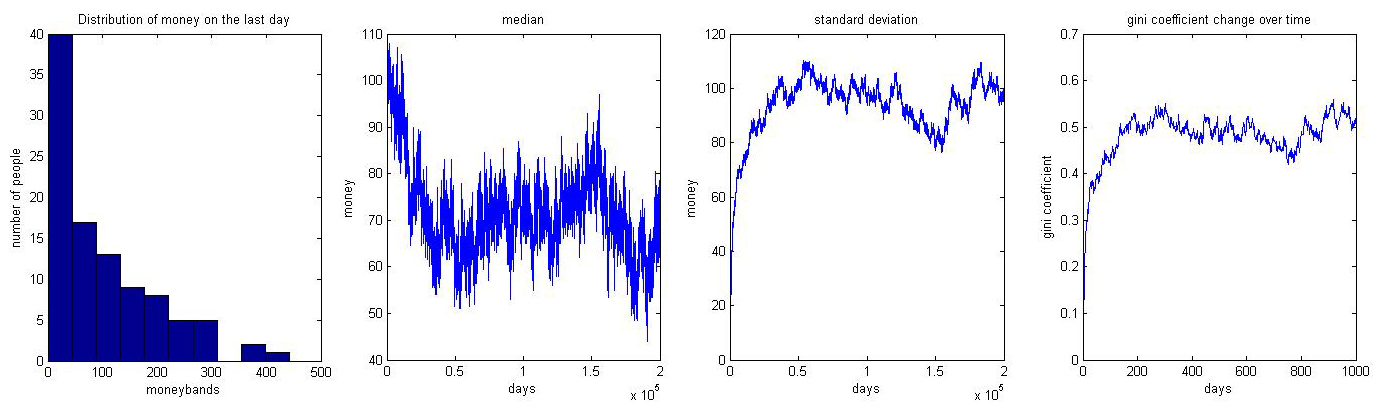
\includegraphics[width=0.9\columnwidth]{ChapterABM/figures/simplemoneytest}%
\caption{Zero-intelligence agents exchange finite money, beginning with equal amounts. \label{fig:simplemoneytest}}%
\end{figure}

\begin{itemize}
	\item Optimise each Bundle. This happens in one of two ways:
	\begin{itemize}
	\item A `greedy optimiser' uses the following method - 
\begin{itemize}
\item The greedy optimiser iterates for a set number 
	\item The iteration is initialised by randomly slicing the budget (the best wage), one slice for each Good in the bundle, before beginning the iterations, so that each has a starting guess price. The iterations are:
	\item `Jiggle' the slices, changing their proportionate size slightly.
	\item `Test-spend' those slices on each Good: find out how much could be bought with the current budget slices using the per-unit price for the Good.
	\item Get a utility level for these quantities of goods. The Utility function is logically separate: the Optimiser deals only with this process of random slicing and adjusting.
	\item If the utility level found is the highest so far, keep the current proportion of slices and return to the 'jiggle' point. Else, revert to the previous slice proportions and try again. This has the effect of ratchetting the budget slices (and thus the spend per Good) towards an optimum.
\end{itemize}
	\item{A Bundle is passed directly to a code version of the constrained utility optima described in section \ref{sec:constrained}.}
	\begin{itemize}
	\item{The Good prices and budget are used to directly calculate optimal good amounts. The utility level is then `read back' from those amounts.}
	\end{itemize}
	\end{itemize}
	\item Once each Bundle has an optimum utility, select the Bundle with the highest:
	\begin{itemize}
	\item Take the best wage: this instructs the Firm to pay the Person.
	\item Buy goods in the quantities found optimal by this Bundle.
	\end{itemize}
\end{itemize}

\end{comment}